\documentclass[a4paper, 12pt]{article}
\usepackage[english,serbian]{babel}

\usepackage[]{algorithm2e}
\SetKwInput{KwData}{Algorithm}
    
\usepackage{graphicx}
\graphicspath{{../slike}}

\usepackage{geometry}
\geometry{margin=2cm}

\usepackage{url}
\usepackage{subfig}
\usepackage{amsmath}
\usepackage{enumitem}

\title{\textsc{Univerzitet u Beogradu \\ Matematički fakultet} \\ \vspace{2cm} {\small \textsc{Seminarski rad}} \\ \vspace{0.3cm} Grafovski probabilistički modeli za analizu i predviđanje struktura sekvenci i njihove primene u bioinformatici \\} 
\date{}

\begin{document}

\maketitle
\thispagestyle{empty}

\vspace{8cm}

\begin{minipage}[t]{5cm}
\textit{Autori:} \\
\textsc{Lazar Vasović}\\
\textsc{Nevena Ćirić}\\
\end{minipage}
\hfill
\begin{minipage}[t]{5cm}
\hglue0.00001pt\hfill  \textit{Profesor:} \\
\hglue0.00001pt\hfill  \textsc{prof. dr Gordana}\\
\hglue0.00001pt\hfill  \textsc{Pavlović-Lažetić} \\
\end{minipage}

\vspace{2cm}

\begin{center}
Beograd, 2022.
\end{center}

\newpage

\section{Vrste grafovskih probabilističkih modela}

Probabilistički modeli se često mogu predstaviti grafovima koji opisuju međusobne zavisnosti između slučajnih promenljivih koje se modeluju. Kako su biološki procesi po prirodi probabilistički, mnogi grafovski probabilistički modeli pronalaze primenu u bioinformatici.

Prema tipu raspodele koju modeluju i strukturi grafa, mogu se uočiti različite vrste grafovskih probabilističkih modela. Na slici 1 prikazano je nekoliko vrsta grafovskih probabilistickih modela koji imaju primenu u bioinformatici i njihovi odnosi u nekoliko aspekata.

\begin{figure}[h!]
    \centering
    \vspace{0.3cm}
    \subfloat{{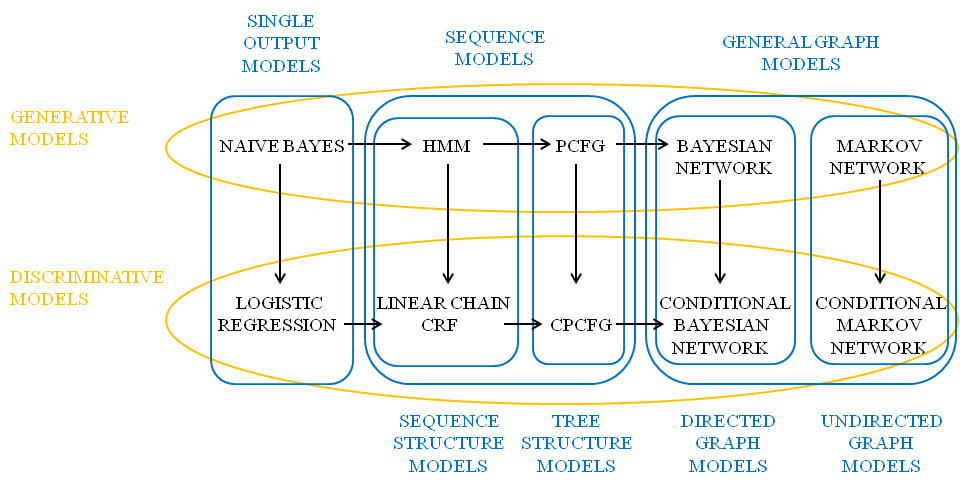
\includegraphics[width=17cm]{PGM}}}
    \vspace{0.15cm}
    \caption{Vrste grafovskih probabilističkih modela}
    \vspace{0.3cm}
\end{figure}

Osnovna podela probabilističkih modela je prema tipu raspodele koju modeluju -- na \textit{generativne} i \textit{diskriminativne modele}. Generativni probabilistički modeli modeluju zajedničku raspodelu svih slučajnih promenljivih od interesa. Diskriminativni probabilisticki modeli modejlu uslovnu raspodelu izlaznih (ciljnih) slučajnih promenljivih za date vrednosti ulaznih (opaženih) slucajnih promenljivih.

Grafovski probabilistički modeli određuju familije raspodela verovatnoće koje se faktorišu prema odgovarajućem grafu. U zavisnosti od toga da li se radi o usmerenom ili neusmerenom grafu, imamo podelu na \textit{Bajesovske mreže} i \textit{Markovljeve mreže}. Ove dve vrste modela razlikuju se u tipu međuzavisnosti između slučajnih promenljivih koje mogu da opišu. 

Bajesovske i Markovljeve mreže u opštem slučaju modeluju zajedničku raspodelu, ali se za opažene vrednosti nekih slučajnih promenljivih mogu prilagoditi tako da modeluju uslovnu raspodelu u odnosu na date promenljive. Ista reprezentacija i parametrizacija može se iskoristiti za modelovanje uslovne raspodele tako što se raspodele pridružene faktorima renormalizuju u odnosu na fiksirane vrednosti opaženih slučajnih promenljivih. Tada govorimo o \textit{uslovnim Bajesovskim} i \textit{Markovljevim mrežama}\footnote{Uslovne Markovljeve mreže se u delu literature nazivaju \textit{uslovna slučajna polja} (eng. CRFs -- Conditional Random Fields). Međutim, mi ćemo pod uslovnim slučajnim poljima podrazumevati sve modele koji uslovnu raspodelu faktorišu prema nekom grafu. Drugim rečima, u terminologiji koju koristimo pod uslovna slučajna polja potpadaju i uslovne Bajesovske mreže.}. Detaljno o ovim modelima može se pročitati u [3].

Sekvencijalni probabilistički modeli su vrsta probabilističkih modela kod kojih su izlazne (neopažene, skrivene) slučajne promenljive međusobno zavisne na taj način da čine sekvencu. Bajesovske mreže, kao usmereni grafovski modeli, mogu da modeluju ovakve međuzavisnosti izlaznih slučajnih promenljivih. 

Specijalni slučaj Bajesovskih mreža koje imaju strukturu stabla i čije izlazne slučajne promenljive čine sekvencu nazivaju se \textit{PCFGs} (eng. Probabilistic Context Free Grammars). Uslovljene varijante ovih modela nazivaju se \textit{CPCFGs} (eng. Conditional Probabilistic Context Free Grammars). 

PCFGs čije grafovske strukture predstavljaju degenerisano stablo, odnosno imaju sekvencijalnu strukturu, nazivaju se \textit{HMMs} (eng. Hidden Markov Models). Njihove uslovljene varijante nazivaju se \textit{linear chain CRFs}.

Kao specijalan slučaj HMM modela koji imaju samo jednu izlaznu slučajnu promenljivu, ali složen skup opažanja (atributa), može se videti model \textit{naivni Bajesov klasifikator}, a kao uslovljena varijanta naivnog Bajesovog klasifikatora model \textit{multinomijalne logističke regresije} (to uključuje i binarni slučaj). Formalni dokaz diskriminatorno-generativne veze između modela logističke regresije i Naivnog Bajesa može se naći u [2].

Dalje će detaljnije biti razmatrani samo sekvencijalni grafovski probabilistički modeli i kako se oni uklapaju u opštu teoriju modelovanja sekvenci. Modeli sekvenci su važni u bioinformatici (računarskoj biologiji) zato što se njima opisuju strukture poput DNK i RNK (sekvence nukleobaza), ali i proteina (sekvenca aminokiselina). U obradi prirodnih jezika (računarskoj lingvistici), analogno se modeluju reči kao sekvence karaktera i rečenice kao sekvence reči.

\section{Sistematizacija modela struktura sekvenci}

Najjednostavnija struktura sekvenci podrazumeva postojanje susednih zavisnosti između elemenata sekvenci -- vrednost $i$-tog elementa sekvence zavisi od vrednosti $(i-1)$-og elementa sekvence. Kompleksnije strukture sekvenci uključuju dugoročne zavisnosti između pojedinačnih elemenata sekvenci, zavisnosti jednog elemenata od više prethodnih elementa sekvenci, kao i njihove kombinacije.

Opštu teoriju modelovanja struktura sekvenci formalizovali su računarski lingvisti kroz \textit{teoriju formalnih jezika i gramatika}.  Formalne gramatike su razvijene u mahom neuspelom pokušaju da precizno okarakterišu strukturu prirodnih jezika. Kasnije su postale važne u teorijskom računarstvu zato što se programski jezici, za razliku od prirodnih jezika, mogu precizno okarakterisati pomoću konačnog skupa pravila. Danas formalne gramatike imaju široku primenu u različitim oblastima, između ostalog i u molekularnoj biologiji za analizu bioloških sekvenci.

\subsection{Hijerarhija Čomskog}

Formalne gramatike se definišu konačnim skupom simbola i pravila izvođenja $\alpha \rightarrow \beta$, gde su $\alpha$ i $\beta$ nizovi simbola. Postoje dve vrste simbola -- apstraktni \textit{neterminalni (nezavršni)} simboli i \textit{terminalni (završni)} simboli koji se pojavljuju u sekvencama (rečima) odgovarajućeg formalnog jezika. Leva strana pravila izvođenja $\alpha$ sadrži najmanje jedan neterminalni simbol kome se desnom stanom pravila izvođenja $\beta$ pridružuje neki niz terminalnih i neterminalnih simbola. Kako bismo ih jasno razlikovali, koristićemo mala slova za terminalne, a velika za neterminalne simbole.
 
Čomski definiše četiri tipa strukture pravila izvođenja gramatika. Rezultujuće četiri klase formalnih gramatika, koje se sastoje samo od pravila izvođenja odgovarajućeg tipa, čine hijerarhiju poznatu kao \textit{hijerarhija Čomskog}. Na slici 2 prikazane su ove četiri klase gramatika, ugnežđene prema restriktivnosti njihovih pravila izvođenja, a samim tim i odnosu skupova jezika koje te gramatike mogu da opišu. Takođe, ova hijerarhija odražava mogućnost gramatika da opišu različite vrste međuzavisnosti elemenata sekvenci, odnosno struktura sekvenci.

Koristićemo sledeće oznake: $W$ za bilo koji neterminalni simbol, $a$ za bilo koji terminalni simbol, $\alpha$ i $\gamma$ za bilo koji niz neterminalnih i/ili terminalnih simbola, uključujući i prazan niz, a $\beta$ za bilo koji neprazan niz neterminalnih i/ili terminalnih simbola.

\begin{figure}[h!]
    \centering
    \subfloat{{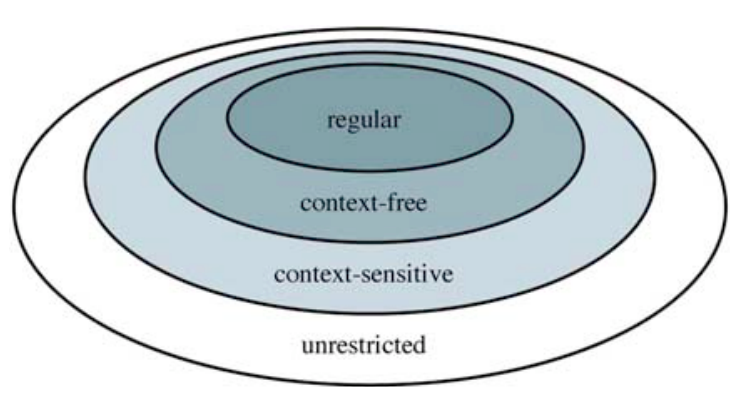
\includegraphics[width=8.7cm]{Chomsky}}}
    \vspace{0.15cm}
    \caption{Hijerarhija Čomskog}
    \vspace{0.15cm}
\end{figure}

\noindent \textbf{Regularne gramatike} \hspace{0.3cm} Dozvoljena su samo pravila izvođenja oblika $W \rightarrow aW$ ili $W \rightarrow a$. Na osnovu strukture pravila izvođenja sledi da regularne gramatike generišu (izvode) sekvence isključivo sleva nadesno. To su najrestriktivnije i najjednostavnije gramatike koje mogu da opišu samo najjednostavnije međuzavisnosti elemenata sekvenci -- zavisnost sledećeg elementa od prethodnog. 

\vspace*{0.2cm}
\noindent \textbf{Kontekstno-slobodne gramatike} \hspace{0.3cm} Sva pravila izvođenja su oblika $W \rightarrow \beta$. Leva strana pravila izvođenja mora biti isključivo jedan neterminalni simbol, dok desna strana pravila nema restrikcija. Desna strana stoga može da generiše korelisani par terminalnih simbola (elemenata sekvence) iz jednog neterminalnog simbola, za razliku od regularnih gramatika kod kojih se par terminalnih simbola mora generisati nezavisno iz dva koraka (pravila izvođenja). Drugim rečima, u odnosu na regularne gramatike, kontekstno-slobodne gramatike dozvoljavaju dodatna pravila koja omogućavaju modelovanje ugnežđenih, dugoročnih zavisnosti (parova) elemenata sekvenci.

\vspace*{0.2cm}
\noindent \textbf{Kontekstno-osetljive gramatike} \hspace{0.3cm} Pravila izvođenja su oblika $\alpha_1 W \alpha_2 \rightarrow \alpha_1 \beta \alpha_2$. Dakle, izvođenja neterminalnih simbola ($W$) zavise od njegovog konteksta ($\alpha_1$ i $\alpha_2$). To je jednako zahtevu da desna strana pravila sadrži najmanje onoliko simbola koliko i leva strana, što znači da kontekstno-osetljive gramatike nikada ne skraćuju prethodno izvedenu sekvencu. Na osnovu prethodnog, kontekstno-osetljive gramatike dozvoljavaju pravila izvođenja oblika $AB \rightarrow BA$\footnote{Pravilo $AB \rightarrow BA$ može se zameniti nizom pravila oblika $\alpha_1 W \alpha_2 \rightarrow \alpha_1 \beta \alpha_2$: $AB \rightarrow XB$, $XB \rightarrow XY$, $X \rightarrow B$, $Y \rightarrow A$. Ako se simboli $X$ i $Y$ ne pojavljuju u drugim pravilima izvođenja, dobija se ekvivalentna gramatika kao ona koja sadrži pravilo $AB \rightarrow BA$.}. Pravila izvođenja ovog oblika se nazivaju \textit{pravila preuređivanja} i ona omogućavaju ukrštanje interakcija između parova simbola terminalnih simbola. Drugim rečima, u odnosu na niže pozicionirane gramatike, kontekstno-osetljive dozvoljavaju dodatna pravila koja omogućavaju modelovanje svih vrsta zavisnosti parova elemenata sekvenci.

\vspace*{0.2cm}
\noindent \textbf{Gramatike bez restrikcija} \hspace{0.3cm} Ni leva ni desna strana pravila izvođenja nemaju restrikcije, odnosno oblika su $\alpha_1 W  \alpha_2 \rightarrow \gamma$. 

\subsection{Automati}

Svaka od klasa formalnih gramatika ima odgovarajući apstraktni računarski formalizam koji se naziva \textit{automat}. Automati su apstraktne mašine kojima se kao ulaz prosleđuju sekvence (reči jezika). Automat obrađuje (parsira) sekvencu deo po deo primenjujući pravila gramatike, pritom menjajući stanje u kome se nalazi. U zavisnosti od završnog stanja automata, sekvenca sa ulaza može biti prihvaćena ili odbijena. Shodno tome, automati se često nazivaju \textit{prihvatačkim sistemima}, za razliku od formalnih gramatika koji se nazivaju \textit{generatorskim sistemima}. 

\noindent \textbf{Konačni automati} \hspace{0.3cm} Sastoje se od konačnog broja stanja koja su međusobno povezana prelazima. Stanja odgovaraju neterminalnim simbolima, a prelazi pravilima izvođenja formalnih gramatika. Parsiranje sekvence vrše jedan po jedan simbol. Dakle, klasa jezika koje prepoznaje konačni automat ekvivalentna je klasi jezika koje generišu regularne gramatike.

\vspace*{0.2cm}
\noindent \textbf{Potisni automati} \hspace{0.3cm} Za razliku od konačnih automata, koji ne zahtevaju nikakvu memoriju osim za praćenje trenutnog stanja, potisni automati imaju (ograničenu) pomoćnu memoriju koja funcioniše po principu steka (po čemu je automat i dobio ime). Parsiranje sekvence se vrši tako što se na stek stavi početni neterminalni simbol gramatike. U svakom narednom koraku skida se po jedan simbol sa steka i u zavisnosti od toga da li je neterminalni ili terminalini simbol u pitanju, vrši se jedna od akcija. Za neterminalni simbol traži se pravilo izvođenja koje se može primeniti nad njim u skladu sa trenutnom pozicijom u parsiranju sekvence i na stek se stavlja desna strana odgovarajućeg pravila izvođenja\footnote{Simboli desne stane izvođenja se na stek slažu počev od najdešnjeg simbola.}. A ako se radi o terminalnom simbolu, poredi se sa sledećim simbolom sekvence i ako se slažu napreduje se u parsiranju sekvence, a u suprotnom se prekida parsiranje i odbacuje sekvenca.
Kako ovakav način parsiranja sekvence omogućava uparivanje elemenata sekvence, jasno je da je klasa jezika koje prepoznaje potisni automat ekvivalentna je klasi jezika koje generišu kontekstno-slobodne gramatike.

\vspace*{0.2cm}
\noindent \textbf{Linearno-ograničeni automati} \hspace{0.3cm} Prepoznaju kontekstno-osetljive jezike, tj. klasa jezika koje prepoznaje linearno-ograničeni automat ekvivalentna je klasi jezika koje generišu kontekstno-osetljive gramatike. Kako su kontekstno-osetljive gramatike ograničene tako da leva strana pravila izvođenja ne može biti duža od desne strane, postoji konačan broj mogućih izvođenja za datu sekvencu\footnote{Nijedan međuproizvod izvođenja ne može biti duži od same sekvence.}. Linearno-ograničeni automat je mehanizam za sistematski pretragu unazad kroz sva moguća izvođenja date sekvence sve dok se ili ne dostigne početni neterminalni simbol gramatike ili dok se ne iscrpe sva moguće izvođenja (bez pronalaženja validnog izvođenja). To je apstraktna mašina koja se sastoji od trake podeljene na ćelije (koja predstavlja memoriju mašine) i glave koja može da čita/piše po ćelijama i da se pomera duž trake. Dužina trake je linearno ograničena dužinom sekvence koja se parsira, s obzirom da međuproizvodi izvođenja ne mogu biti duži od date sekvence.

\vspace*{0.2cm}
\noindent \textbf{Tjuringova mašina} \hspace{0.3cm} Ekvivalent su gramatikama bez restrikcija. Tjuringova mašina je suštinski isto što i linearno-ograničeni automat sa neograničenom dužinom trake (memorije).

\subsection{Stohasticke (probabilističke) gramatike}

Svaka od formalnih gramatika iz hijerarhije Čomskog može se koristiti u stohastičkom obliku kao osnova za probabilističke modele struktura sekvenci. Stohastičke gramatike generišu neku sekvencu $x$ sa nekom verovatnoćom $P(x)$, dok nestohastičke gramatike ili mogu da generišu sekvencu $x$ ili ne. Drugim rečima, stohastičke gramatike definišu raspodelu verovatnoća nad sekvencama $x$, tako da $\sum_x P(x) = 1$.

U stohastičkoj varijanti regularnih i kontekstno-slobodnih gramatika zbir verovatnoća svih mogućih pravila izvođenja iz bilo kog neterminalnog simbola mora biti 1. Međutim, pravila izvođenja i njima pridružene verovatnoće za stohastičke verzije kontekstno-osetljivih i gramatika bez restrikcija moraju biti formulisana pažljivije. Potrebno je obezbediti da za svaki kontekst postoji jedinstveno izvođenje. To se postiže definisanjem pravila gramatike tako da kontekst u kome se pojedinačni neterminalni simbol pojavljuje jednoznačno određuje skup mogućih pravila izvođenja koja se u tom slučaju mogu primeniti, odnosno za svaki neterminalni simbol ne postoji više od jedne forme leve strane pravila izvođenja u kome se on pojavljuje\footnote{Npr. gramatika ne sme da ima oba pravila $bW \rightarrow bb$ i $W \rightarrow b$ zato što to ostavlja mogućnost izbora koje će od ova dva pravila biti primenjeno u slučaju kada se $W$ pojavljuje sa kontekstom $b$. A to dovodi do više mogućih izvođenja za jednu sekvencu.}. Zatim, pridruživanjem verovatnoća pravilima izvođenja tako da se sumiraju na 1 za bilo koji neterminalni simbol u svakom mogućem kontekstu, dobija se stohastička gramatika.

Na slici 3 data je tabela koja sistematizuje klase gramatika, njima odgovarajuće analitičke formalizme, stohastičke varijante i diskriminatvne analogone (gramatike su po svojoj prirodi generativne), kao i modele struktura sekvenci koji se na njima zasnivaju (podebljana slova). U nastavku će detaljnije biti razmatrani samo modeli koji se zasnivaju na stohastičkim regularnim i kontekstno-slobodnim gramatikama, jer samo oni imaju praktičnu primenu u bioinformatici.

\begin{figure}[h!]
    \centering
    \vspace{0.15cm}
    \subfloat{{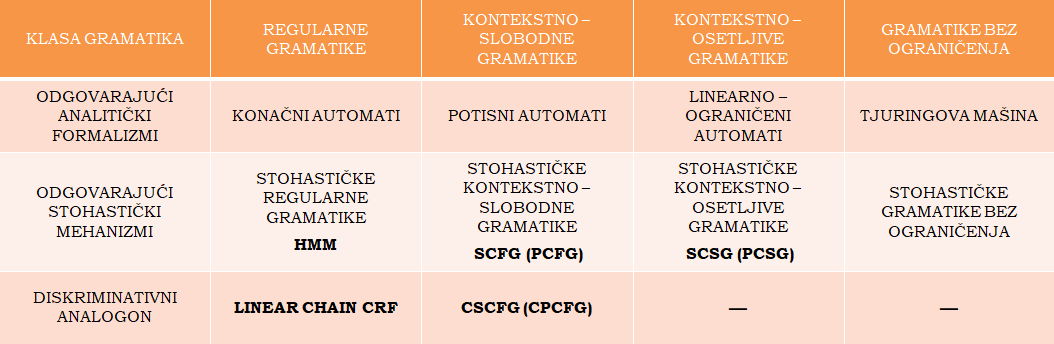
\includegraphics[width=17cm]{sitematizacija}}}
    \vspace{0.2cm}
    \caption{Sistematizacija modela struktura sekvenci}
\end{figure}

\section{HMM}

\textit{HMM} (eng. \textit{Hidden Markov Mode}l) je ekvivalent stohastičkim regularnim gramatikama. Međutim, definisanje stohastičke gramatike je samo prvi korak u kreiranju upotrebljivog modela strukture sekvenci. Pored gramatike, model određuju algoritmi za:

\begin{enumerate}
\item[(1)] određivanje optimalnih vrednosti parametara modela, tj. pridruživanje verovatnoća pravilima izvođenja tako da opisuju strukturu sekvence koja se modeluje,
\item[(2)] poređenje (poravnanje) struktura novih sekvenci prema strukturi sekvence koju dati model modeluje, što odgovara određivanju optimanlnog izvođenja za novu sekvencu,
\item[(3)] kvantifikovanje sličnosti struktura novih sekvenci sa strukturom sekvence koju dati model modeluje, što odgovara izračunavanju verovatnoće da nova sekvenca bude generisana datom gramatikom.
\end{enumerate}

HMM se najčešće predstavlja i definiše kao probabilistički konačni automat, odnosno graf koji se sastoji od konačnog skupa čvorova (stanja) koja su međusobno povezana granama (prelazima) sa pridruženim verovatnoćama. Iz jednog stanja se sa određenom verovatnoćom može preći u drugo stanje, a iz svakog od stanja se po dolasku emituje simbol sekvence sa određenom verovatnoćom. Kako se iz svakog stanja u opštem slučaju može emitovati bilo koji od simbola (sa različitim verovatnoćama), znajući sekvencu nije moguće odrediti koji simbol je generisan iz kog stanja. Otuda potiče naziv modela -- sekvenca stanja iz kojih je generisana sekvenca simbola je \textit{skrivena}.

\newpage
\noindent Dakle, HMM je određen grafom (skupom stanja i prelaza) i sledećim skupom parametara:

\begin{itemize}[itemsep=-0.03ex]
\renewcommand\labelitemi{\small$\bullet$}
\vspace*{-0.1cm}
\item $a_{kl}$ -- verovatnoće prelaska iz stanja $k$ u stanje $l$ 
\item $e_k(b)$ -- verovatnoće emitovanja simbola $b$ iz stanja $k$
\vspace*{-0.1cm}
\end{itemize}

\noindent Kako bi se jasnije razlikovalo kada se govori o sekvencama simbola a kada o sekvencama stanja, sekvence simbola se radije nazivaju \textit{putanjama} (kroz graf stanja), dok se sekvence simbola nazivaju kraće samo \textit{sekvencama}. Neka su sa $x_i$ označeni elementi sekvenca, a sa $\pi_i$ elementi putanja, i neka je sa $0$ označeno početno stanje modela (automata). Tada se zajednička raspodela sekvence $x$ i njoj odgovarajuće putanje $\pi$ može dobiti kao

$$P(x, \pi) = a_{0\pi_1}\prod_{i=1}^{L} e_{\pi_i}(x_i) a_{\pi_i\pi_{i+1}}$$ 

\noindent gde je $L$ dužina date sekvence. Kako putanja u većini slučajeva nije poznata, a upravo je ona od interesa\footnote{Stanja modela su ta koja opisuju strukturu sekvence u nekom smislu (unutar/van CpG ostrva, fer/nefer kockica, match/insetrion/deletion poravnanje elemenata dve sekvence itd.).}, od svih mogućih putanja najsmislenije je odabrati onu optimalnu -- za koju se dobija najveća vrednost zajedničke verovatnoće 

$$\pi^* = \underset{\pi}{argmax} P(x, \pi)$$

\noindent Optimalna putanja $\pi^*$ može se odrediti rekurzivno, dinamičkim programiranjem. Pretpostavimo da su poznate verovatnoće $v_k(i)$ optimalne putanje za deo sekvence do $(i-1)$-og elementa (uključujući i njega), a koje se završavaju u stanju $k$. Tada se verovatnoća optimalne putanje za deo sekvence zaključno do $i$-tog elementa, a koja se završava u stanju $l$ može izračunati kao

$$v_l(i) = e_l(x_i)\underset{k}{max}(v_k(i-1)a_{kl})$$   

\noindent Kako svaka putanja podrazumevano kreće iz stanja $0$ (početno stanje), tada je $v_0(0) = 1$ i $v_k(0) = 0$ za sva stanja $k \neq 0$ (izlazak iz rekurzije). Čuvanjem pokazivača unazad, optimalna putanja se može dobiti pomoću backtracking-a. Kompletan algoritam je prikazan u nastavku.

\begin{algorithm}[h!] 
 \KwData{\textbf{Viterbi}}
 \vspace*{0.2cm}
 Initialization ($i=0$): \hspace{0.3cm} $v_0(0) = 1$, $v_k(0) = 0$ for $k \neq 0$ \\
 \vspace*{0.2cm}
 Recursion ($i=1, ..., L$): \hspace{0.05cm}$v_l(i) = e_l(x_i)\max_k(v_k(i-1)a_{kl})$ \\
 \hspace*{4.25cm} $ptr_i(l) = argmax_k (v_k(i-1)a_{kl})$ \\
 \vspace*{0.2cm}
 Termination: \hspace{1.8cm} $P(x, \pi^*) = \max_k (v_k(L)a_{k0})$ \\
 \hspace*{4.25cm} $\pi_L^* = argmax_k(v_k(L)a_{k0})$ \\
 \vspace*{0.2cm}
 Traceback ($i=L, ..., 1)$: \hspace{0.05cm}$\pi_{i-1}^* = ptr_i(\pi_i^*)$           
\end{algorithm}

Ukoliko želimo da odredimo kolika je verovatnoća da neka sekvenca $x$ bude generisana datim modelom, tada treba uzeti u obzir sve moguće putanje

$$P(x) = \sum_{\pi}P(x, \pi)$$

\noindent Kako broj mogućih putanja $\pi$ eksponencijalno raste sa dužinom sekvence, izračunavanje $P(x)$ nabrajanjem svih mogućih putanja i računajem ponaosob $P(x, \pi)$ nije praktično primenljiv (biološke sekvence su najčešće veoma dugačke). Drugi pristup je da se ukupna verovatnoća generisanja sekvence $x$ izračunava rekurzivno, računajući verovatnoće da delovi sekvence sve do $i$-tog elementa budu generisani modelom. To se može postići algoritmom koji je analogan Viterbijevom algoritmu, s tim što se umesto maksimuma računa zbir. Ovaj algoritam se naziva \textit{algoritmom unapred}.

\begin{algorithm}[h!] 
 \KwData{\textbf{Forward algorithm}}
 \vspace*{0.2cm}
 Initialization ($i=0$): \hspace{0.3cm} $f_0(0) = 1$, $v_k(0) = 0$ for $k \neq 0$ \\
 \vspace*{0.2cm}
 Recursion ($i=1, ..., L$): \hspace{0.05cm}$f_l(i) = e_l(x_i)\sum_k f_k(i-1)a_{kl}$ \\
 \vspace*{0.2cm}
 Termination: \hspace{1.8cm} $P(x) = \sum_k f_k(L)$ \\
\end{algorithm}

\noindent Isto to se može postići izračunavanjem verovatnoća da delovi sekvence od $i$-tog do poslednjeg elementa budu generisani modelom. Tako definisan algoritam naziva se \textit{algoritmom unazad}.

\begin{algorithm}[h!] 
 \KwData{\textbf{Backward algorithm}}
 \vspace*{0.2cm}
 Initialization ($i=L$): \hspace{1cm} $b_k(L) = 1$ for all $k$ \\
 \vspace*{0.2cm}
 Recursion ($i=L-1, ..., 1$): \hspace{0.05cm}$b_k(i) = \sum_k a_{kl}e_l(x_{i+1})b_l(i+1)$ \\
 \vspace*{0.2cm}
 Termination: \hspace{2.5cm} $P(x) = \sum_l a_{0l}e_l(x_1)b_l(1)$ \\
\end{algorithm}

Prethodno navedena tri algoritma zapravo predstavljaju deo samog modela HMM. Viterbijev algoritam odgovara stavki (2), a algoritmi unapred i unazad stavki (3) sa početka poglavlja. Ostaje još da vidimo na koji način se dolazi do optimalnih vrednosti parametara HMM modela (stavka (1)).

Kao što je bilo lakše izračunati verovatnoću generisanja sekvence kada joj je putanja poznata, isto tako je lakše oceniti parametre modela kada su poznate putanje za sve trening sekvence. Kada su putanje poznate može se izbrojati koliko puta je svaki od prelaza korišćen, kao i koliko puta je koji simbol emitovan iz svakog od stanja. Neka su sa $A_{kl}$ i $E_k(b)$ označene redom te vrednosti. Tada se vrednosti parametara modela $a_{kl}$ i $e_k(b)$ mogu oceniti metodom maksimalne verodostojnosti kao

\begin{equation}\label{eq:pythagoras}
a_{kl} = \frac{A_{kl}}{\sum_{l'}A_{kl'}}  \hspace{1.5cm}  e_k(b) = \frac{E_k(b)}{\sum_{b'}{E_k(b')}}
\end{equation}

Kada putanje nisu poznate ne postoji direktna jednačina za ocenu vrednosti parametara, već se mora koristiti neki oblik iterativne procedure (optimizacioni algoritam). \textit{Baum-Welch algoritam} iterativno ocenjuje $A_{kl}$ i $E_k(b)$ na osnovu trenutnih vrednosti $a_{kl}$ i $e_k(b)$ uzimajući u obzir sve moguće putanje za svaku od trening sekvenci, a zatim na osnovu jednačina (1) izračunava nove vrednosti za $a_{kl}$ i $e_k(b)$. Preciznije, $A_{kl}$ i $E_k(b)$ se izračunavaju kao očekivani broj odgovarajućih prelaza i emisija koji su korišćeni za generisanje datog skupa trening sekvenci. Verovatnoća da je prelaz $k \rightarrow l$ korišćen na $i$-toj poziciji za sekvencu $x$ može se dobiti kao

$$P(\pi_i = k, \pi_{i+1} = l | x) = \frac{P(\pi_i = k, \pi_{i+1} = l, x)}{P(x)} = \frac{f_k(i)a_{kl}e_l(x_{i+1})b_l(i+1)}{P(x)}$$

\noindent Sumiranjem po svim pozicijama $i$ i svim trening sekvencama $x^j$ dobija se ocena za $A_{kl}$, tj.

\begin{equation}\label{eq:pythagoras}
A_{kl} = \sum_{j}\frac{1}{P(x^j)}\sum_{i}f_k^j(i)a_{kl}e_l(x_{i+1}^j)b_l^j(i+1)
\end{equation}

\noindent Na sličan način se dolazi i do očekivanog broja emisija simbola $b$ iz stanja $k$ za date trening sekvence

\begin{equation}\label{eq:pythagoras}
E_k(b) = \sum_{j}\frac{1}{P(x^j)}\sum_{i|x_i^j=b}f_k^j(i)b_k^j(i)
\end{equation}

\noindent Na osnovu ovako dobijenih vrednosti $A_{kl}$ i $E_k(b)$ izračunavaju se nove ocene parametametara modela pomoću jednačina (1). Iteriranje se vrši sve dok se ne ispuni neki (zadati) kriterijum zaustavljanja ili dok se ne dostigne neki unapred određeni broj iteracija. Tipično se za kriterijum zaustavljanja uzima kada promena vrednosti parametara modela iz iteracije u iteraciju postane manja od nekog unapred zadatog praga.
Kompletan algoritam je prikazan u nastavku:

\begin{algorithm}[h!] 
 \KwData{\textbf{Baum-Welch}}
 \vspace*{0.2cm}
 Initialization: pick arbitrary model parameters \\
 \vspace*{0.2cm}
 Recurrence: \hspace{0.25cm} set all the $A$ and $E$ variables to zero \\
 	     \hspace{2.5cm} for each sequence j = 1...n \\
             \hspace{3.3cm} calculate $f_k(i)$ for $j$-th sequence using the forward algorithm \\
             \hspace{3.3cm} calculate $b_k(i)$ for $j$-th sequence using the backward algorithm \\
             \hspace{3.3cm} add the contribution of $j$-th sequence to $A$ (2) and $E$ (3) \\
             \hspace{2.5cm} calculate the new model parameters using (1) \\ 
 \vspace*{0.2cm}
 Termination: \hspace{0.05cm} stop if the change in model parameters value is lass than some \\
              \hspace{2.5cm} predefined treshold or the maximum number of iterations is exceeded \\
\end{algorithm}

Često se kao alternativa Baum-Welch algoritmu koristi tzv. \textit{Viterbijevo učenje}. U ovom pristupu se do ocena za $A_{kl}$ i $E_k(b)$ dolazi na osnovu optimalnih putanja trening sekvenci dobijenih pomoću Viterbijevog algoritma za tekuće vrednosti parametara modela. Zatim se na isti način vrši izračunavanje novih vrednosti parametara modela. Ovi koraci se ponavljaju sve dok ima promena u optimalnim putanjama koje se dobijaju za trening sekvence. \\

HMM modeli imaju široku primenu, kako u bioinformatici tako i u mnogim drugim oblastima. Najvažnija primena HMM u bioinformatici je za modelovanje primarne strukture pojedinačnih sekvenci i familija sekvenci, odnosno za jednostruko i višestruko poravnanje sekvenci. Na slici 4 prikazane su strukture HMM modela za jednostruko i višestruko poravnanje sekvenci - tzv. \textit{pair HMM} i \textit{profile HMM} modeli. Stanja $M$, $I$ i $D$  modeluju redom poklapanja (eng. matches), insercije i delecije simbola nove sekvence u odnosu na odgovarajuće simbole trening sekvence. Razlika profile HMM u odnosu na pair HMM je samo u tome što se kod profile HMM svaka pozicija poravnanja modeluje odvojenim skupom stanja $M$, $I$ i $D$.

\begin{figure}[h!]
  \centering
  \vspace{-0.1cm}
  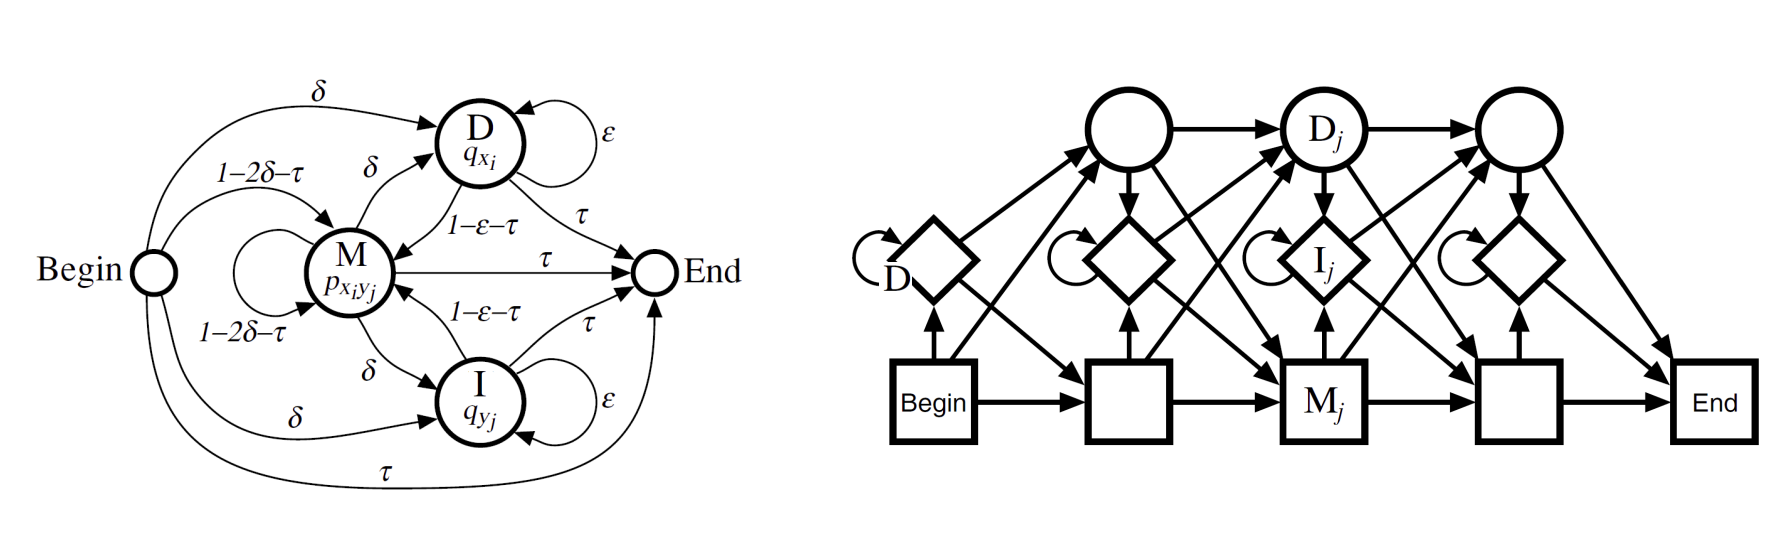
\includegraphics[width=0.96\textwidth]{HMM}
  \caption{Struktura \textit{pair HMM} na levoj strani i \textit{profile HMM} na desnoj}
\end{figure}

\newpage
\section{SCFG modeli}

Za razliku od primarne strukture, modelovanje sekundarne strukture mnogih bioloških sekvenci zahteva modelovanje ugnežđenih, dugoročnih zavisnosti elemenata sekvenci. Kao što je ranije rečeno, kontekstno-slobodne gramatike modeluju upravo ovakvu vrstu međuzavisnosti. Pandan HMM modelima su tzv. \textit{SCFG modeli}, modeli koji se zasnivaju na stohastičkim kontekstno-slobodnim gramatikama.

Isto kao HMM modeli, i SCFG modeli su pored gramatike određeni algoritmima (1), (2) i (3) sa početka poglavlja 3. Pre nego što damo opise ovih algoritama uvešćemo pojmove stabala parsiranja i normalne forme kontekstno-slobodnih gramatika.

\subsection{Stabla parsiranja}

Kod kontekstno-slobodnih gramatika, izvođenja (parsiranja) sekvenci imaju strukturu stabla, kao na slici 5. Početni neterminalni simbol gramatike odgovara korenu stabla, ostali neterminalni simboli unutrašnjim čvorovima, a terminalni simboli (elementi sekvence) listovima stabla. Grane između čvorova odgovaraju pravilima izvođenja, tj. potomci unutrašnjih čvorova (neterminalnih simbola) su čvorovi koji odgovaraju simbolima desne stane izvođenja za te neterminalne simbole.

\begin{figure}[h!]
  \centering
  \vspace{0.05cm}
  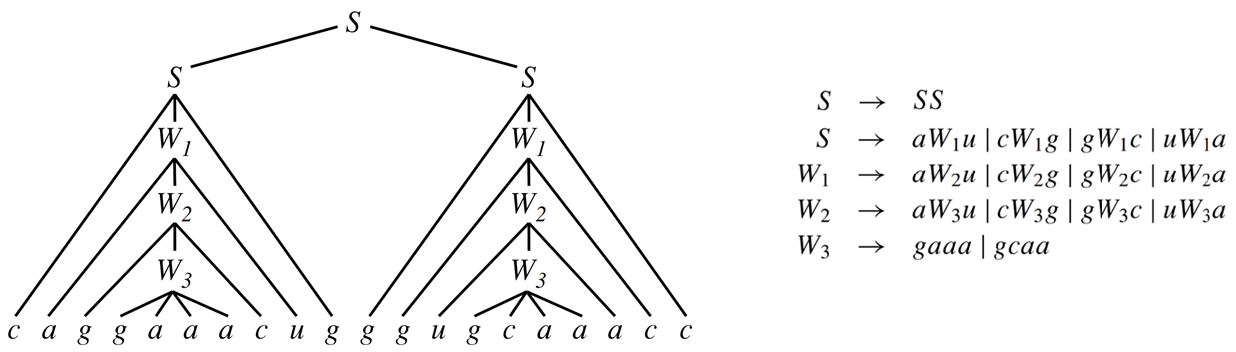
\includegraphics[width=0.99\textwidth]{parsiranje}
  \caption{Primer stabla parsiranja RNK sekvence u odnosu na gramatiku na desnoj strani}
\end{figure}

Svako podstablo stabla parsiranja odgovara izvođenju nekog kontinualnog segmenta posmatrane sekvence. Ovo svojstvo stabala parsiranja je veoma važno zato što omogućava algoritmima da grade optimalna stabla parsiranja (tj. izvođenja) za sekvencu rekurzivno izgrađujući sve veća i veća optimalna podstabla parsiranja za sve veće i veće podsekvence.

\subsection{Normalna forma kontekstno-slobodnih gramatika}

Kako desna strana pravila izvođenja kod kontekstno-slobodnih gramatika može imati proizvoljnu formu, da bi se mogli formulisati opšti algoritmi za parsiranje sekvenci, potrebno je nametnuti neku vrstu normalne forme za pravila izvođenja. Jedna takva normalna forma je \textit{normalna forma Čomskog}, koja zahteva da su sva pravila izvođenja oblika $W_v \rightarrow W_yW_z$ ili $W_v \rightarrow a$. Svaka kontekstno-slobodna gramatika se može transformisati u normalnu formu zamenom pojedinačnih pravila izvođenja (koja nisu u normalnoj formi) nizom pravila izvođenja odgovarajućeg oblika iz dodatnih neterminalnih simbola. Na primer, pravilo izvođenja $S \rightarrow aSu$ se može zameniti pravilima $S \rightarrow W_1W_2$, $W_1 \rightarrow a$, $W_2 \rightarrow SW_3$ i $W_3 \rightarrow u$ uvođenjem novih neterminalnih simbola $W_1$, $W_2$ i $W_3$. Dakle, svi algoritmi koji se definišu za kontekstno-slobodne gramatike u normalnoj formi Čomskog generalno su primenjivi na bilo koju kontekstno-slobodnu gramatiku. Naravno, algoritme je moguće prilagoditi tako da rade i bez normalizacije ulazne gramatike.

\subsection{Algoritmi SCFG modela}

Prvo ćemo uvesti notaciju koja ce biti korišćena prilikom definisanja algoritama. Posmatramo stohastičku kontekstno-slobodnu gramatiku u normalnoj formi Čomskog sa skupom neterminalnih simbola \{$W_1$, ..., $W_M$\}, gde je sa $W_1$ označen početni neterminal. Pravila izvođenja su, dakle, oblika $W_v \rightarrow W_yW_z$ ili $W_v \rightarrow a$. Neka su verovatnoće pridružene ovim pravilima izvođenja (verovatnoća tranzicije iz stanja $W_v$ u stanja $W_y$ i $W_z$ i verovatnoća emisije simbola $a$ iz stanja $W_v$) označene redom sa $t_v(y, z)$ i $e_v(a)$. I neka je sa $x = x_1....x_L$ označena sekvenca koja se parsira.

\textit{Algoritam iznutra} izračunava verovatnoću $\alpha(i, j, v)$ stabla parsiranja za podsekvencu $x_i...x_j$ sa korenom u $W_v$. Izračunavanje počinje od podsekvenca dužine 1 ($i = j$) i rekurzivno ide ka sve dužim i dužim podsekvencama, sve dok se ne odredi verovatnoća stabla parsiranja za kompletnu sekvencu sa korenom u $W_1$. U nastavku je prikazan kompletan algoritam, kao i shematska ilustracija rekurzivnog koraka algoritma.

\begin{figure}[h!]
  \centering
  \vspace{-0.4cm}
  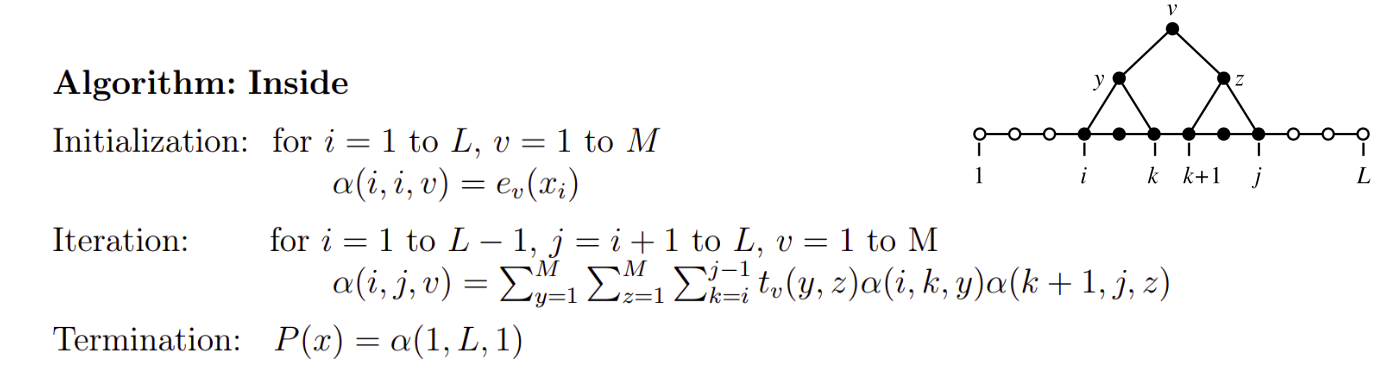
\includegraphics[width=\textwidth]{inside}
\end{figure}

Dakle, algoritam iznutra izračunava ukupnu verovatnoću parsiranja (izvođenja) sekvence $x$, uzimajući u obzir sva moguća stabla parsiranja (izvođenja) za datu sekvencu. Isto to se može dobiti \textit{algoritmom spolja} koji rekurzivno izračunava verovatnoću $\beta(i, j, v)$ stabla parsiranja za sekvencu $x$ sa korenom u $W_1$ ($S$), a isključujući sva podstabla sa korenom u $W_v$ koja generišu podsekvencu $x_i...x_j$. Izračunavanje počinje od najveće isključene podsekvence $x_1...x_L$ i rekurzivno ide ka isključivanju sve kraćih podsekvenci, sve dok se ne odredi verovatnoća stabla parsiranja za kompletnu sekvencu $x$. Kompletan algoritam je prikazan u nastavku.

\begin{figure}[h!]
  \centering
  \vspace{-0.2cm}
  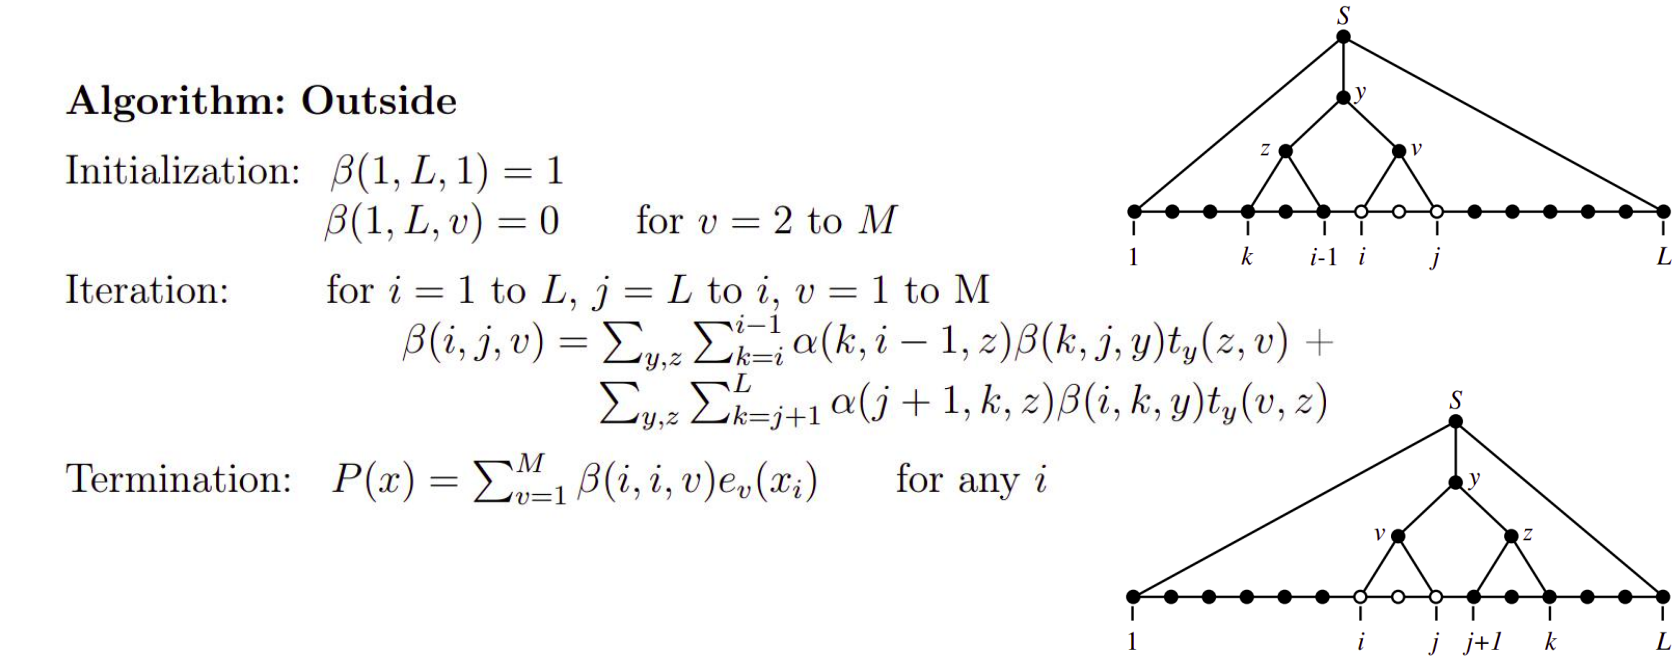
\includegraphics[width=\textwidth]{outside}
\end{figure}


Algoritmi iznutra i spolja za SCFG modele su pandan algoritmima unapred i unazad za HMM modele. Kao što je Baum-Welch algoritam za određivanje optimalnih parametara HMM modela definisan pomoću algoritama unapred i unazad, slično se pomoću algoritama iznutra i spolja definiše algoritam za određivanje optimalnih parametara SCFG modela. Zbog svoje kompleksnosti i rogobatnog zapisa, ovaj algoritam neće biti prikazan na ovom mestu.

\newpage

Pandan Viterbijevom algoritmu za HMM modele je \textit{CYK (Cocke-Younger-Kasami) algoritam} za SCFG modele koji pronalazi optimalno stablo parsiranja za datu sekvencu. CYK algoritam izračunava verovatnoću $\gamma(i, j, v)$ optimalnog stabla parsiranja za podsekvencu $x_i...x_j$ sa korenom u $W_v$. Pored toga, čuvaju se tzv. \textit{traceback} promenljive $\tau(y, z, k)$ koje zapravo predstavljaju trojke $(y, z, k)$ potrebne za rekonstrukciju optimalnog stabla parsiranja. U nastavku je prikazan algoritam CYK, a zatim i \textit{CYK traceback algoritam} koji tehnikom bektrekinga i korišćenjem pomoćne memorije u vidu steka rekonstruiše optimalno stablo parsiranja.

\begin{algorithm}[h!] 
 \KwData{\textbf{CYK}}
 \vspace*{0.2cm}
 Initialization: \hspace{0.01cm} for $i = 1$ to $L$, $v = 1$ to $M$ \\
 		 \hspace{3.3cm} $\gamma(i, i, v) = e_v(x_i)$ \\
 		 \hspace{3.3cm} $\tau(i, i, v) = (0, 0, 0)$ \\
 \vspace*{0.2cm}
 Iteration:  \hspace{0.71cm} for $i = 1$ to $L - 1$, $j = i + 1$ to $L$, $v = 1$ to $M$ \\
             \hspace{3.3cm} $\gamma(i, j, v) = \underset{y,z}{\max} \underset{i \leq k \leq j-1}{\max} t_v(y, z) \gamma(i, k, y) \gamma(k+1, j, z)$\\
             \hspace{3.3cm} $\tau(i, j, v) = \underset{y, z, i \leq k \leq j-1}{argmax} t_v(y, z) \gamma(i, k, y) \gamma(k+1, j, z)$\\ 
 \vspace*{0.2cm}
 Termination: \hspace{0.11cm} $P(x) = \gamma(1, L, 1)$ \\
\end{algorithm}

\begin{algorithm}[h!] 
 \KwData{\textbf{CYK traceback}}
 \vspace*{0.2cm}
 Initialization: \hspace{0.01cm} push $(1, L, 1)$ on the stack \\
 \vspace*{0.2cm}
 Iteration:  \hspace{0.71cm} pop $(i, j, v)$ \\ 
             \hspace{2.5cm} $(y, z, k) = \tau(i, j, v)$ \\ 
             \hspace{2.5cm} if $\tau(i, j, v) = (0, 0, 0)$ (implying $i = j$) \\
             \hspace{3.3cm}attach $x_i$ as the child of $v$ \\
             \hspace{2.5cm} else \\
             \hspace{3.3cm} attach $y, z$ to parse tree as children of $v$ \\
             \hspace{3.3cm} push $(k+1, j, z)$ \\
             \hspace{3.3cm} push $(i, k, y)$ \\ 
\end{algorithm}


\subsection{Modelovanje sekundarne strukture RNK}

RNK molekuli se tipično sastoje od jednog lanca nukleotidnih baza koji može da se savija intramolekularno i formira segmente uparenih nukleotidnih baza. Bazni parovi $A-U$ i $G-C$ su kanonski (prema Votsonu i Kriku), ali je zastupljen i nekanonski par $U-G$, a u nekim slučajevima su moguća i druga uparivanja. Struktura formiranih baznih parova naziva se \textit{sekundarna struktura RNK}. Na slici 6 prikazan je primer sekundarne strukture RNK molekula.

Za RNK je karakteristicno to da homologne sekvence (istog porekla, sa zajedničkim evolutivnim pretkom) imaju sličnu sekundarnu strukturu, dok im primarne strukture ne moraju imati značajne sličnosti. Drastične promene (mutacije) u primarnoj strukturi sekvenci mogu se tolerisati sve dok kompenzacione mutacije održavaju uparivanja baza na odgovarajućim pozicijama. To znači da sekundarna struktura RNK evoluira (mutira) sporije od primarne strukture, što modele sekundarne strukture čini podesnim za traženje homologija kod RNK sekvenci.

Bazni parovi se skoro uvek javljaju na ugnežđeni način u sekundarnoj strukturi RNK. Kako kontekstno-slobodne gramatike modeluju upravo ovakav tip međuzavisnosti, to čini SCFG modele prikladnim izborom za probabilističko modelovanje sekundarne strukture RNK.

\newpage

\begin{figure}[h!]
    \centering
    \captionsetup{width=0.7\linewidth}
    \vspace{-0.15cm}
    \subfloat{{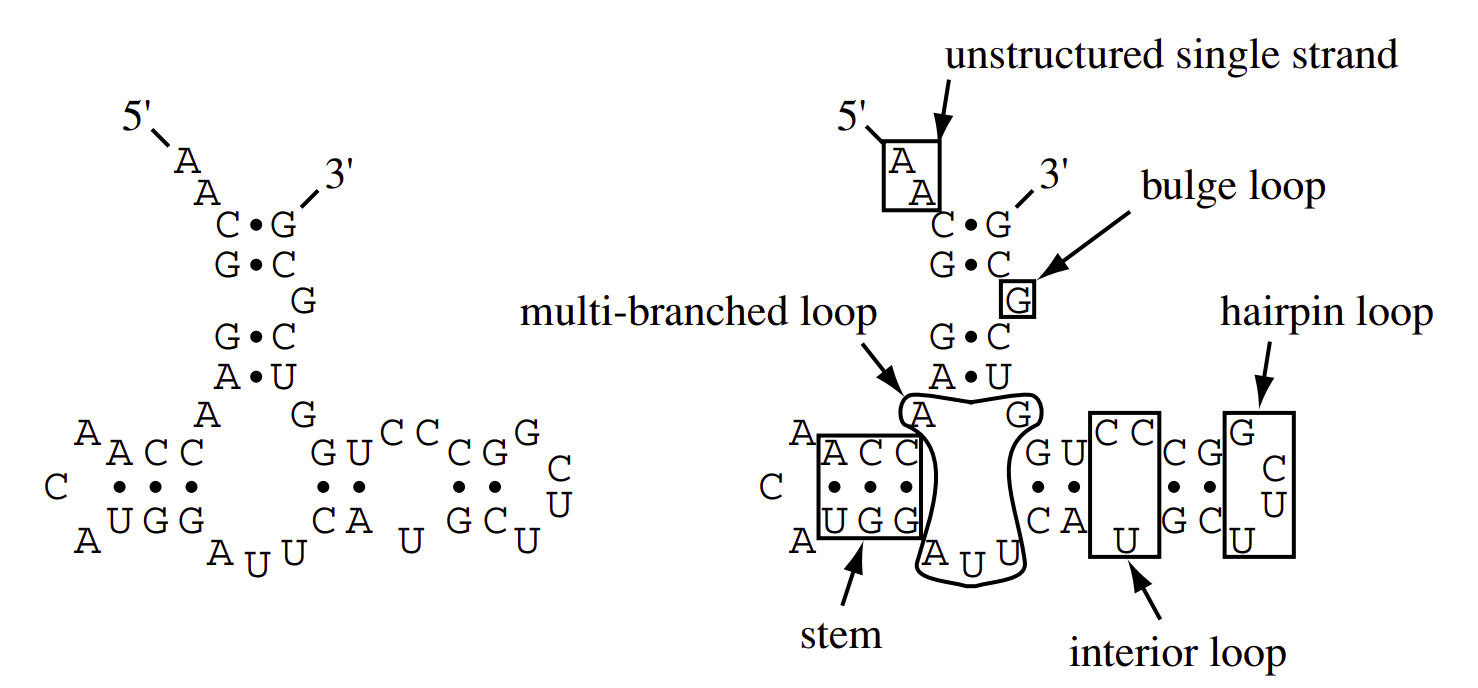
\includegraphics[width=14cm]{RNA}}}
    \vspace{0.1cm}
    \caption{Primer sekundarne strukture RNK zajedno sa uočenim različitim elemenatima te strukture koje treba modelovati}
\end{figure}

Postoje različiti pristupi problemu modelovanja sekundarne strukture RNK sekvenci pomoću SCFG. Jedan mogući pristup je pronalaženje strukture sa najviše baznih parova. \textit{Algoritam Nussinov} i njemu odgovarajući SCFG model imaju upravo ovakav pristup. Mane ovog pristupa su to da ne uzima u obzir važne strukturne karakteristike kao što su preferencije ka određenim dužinama petlji ili preferencije ka određenim kombinacijama susednih baznih parova.

Drugaciji pristup se zasniva na tome da intramolekularno savijanje RNK diktiraju biofizički procesi. Najsofisticiraniji metod za predviđanje sekundarne strukture pojedinačnih RNK sekvenci je \textit{Zukerov termodinamički model} i njemu odgovarajuća SCFG, koji pretpostavljaju da je optimalna struktura ona sa najnižom slobodnom energijom. I algoritam Nusinov i Zukerov algoritam izračunavaju optimane strukture rekurzivno, dinamičkim programiranjem.

Svi PCFG modeli su generativni po prirodi, što znači da modeluju zajedničku raspodelu sekvenci i struktura. Očekivano bi (i intuitivno i formalno) bilo da se bolje ponaša diskriminativni model, koji neposredno maksimizuje uslovnu raspodelu struktura pri sekvenci. Ovakav model naziva se CPCFG i predstavlja logaritamsko-linearni model prema PCFG na isti način na koji je to CRF prema HMM, odnosno logistička regresija (naivni Markov) prema naivnom Bajesu. Ovakav model pridružuje atribute (npr. prefiks podsekvence) pravilima izvođenja, čime pokriva bogatiji skup informacija. Više o ovakvom modelu može se videti u [4] i [5].

Za modelovanje sekundarne strukture familija RNK sekvenci koriste se tzv. \textit{modeli kovarijacije}, kontekstno-slobodni pandan profilnih HMM modela. Za razliku od profilnih HMM modela, koje karakteriše repetitivna linearna arhitektura, kovarijacioni modeli imaju repetitivnu drvoliku arhitekturu, koja je pogodna za modelovanje konsenzusnih sekundarnih stuktura familije RNK sekvenci. Više o ovom i ostalim modelima zasnovanim na PCFG može se pronaći u [1].

Osnovna mana predstavljenih modela je u tome što nisu u stanju da modeluju neugnežđene interakcije između elemenata sekvenci (tzv. \textit{pseudočvorove}). Postoje određeni algoritmi dinamičkog programiranja koji mogu da predvide pojedine tipove pseudočvorova, ali po ceni znatno veće složenosti. Oni se stoga najčešće predviđaju metodama homologije (očekuje se postojanje pseudočvora na istom mestu u srodnim RNK), u koje spadaju i pomenuti kovarijansni modeli.

Postoje i drugačiji pristupi modelovanju sekundarne strukture RNK, čiji se opisi mogu naći u [6]. Savremeni pristup ovom problemu zasnovan je na dubokom učenju, koje je u stanju da uoči najrazličitije vrste međuzavisnosti. Uz pogodan izbor pretpostavki i dovoljno podataka za obučavanje, predviđanja su zadovoljavajuće tačna. Dosad su se najbolje pokazale složene neuronske mreže tipa Bi-LSTM. U budućnosti se očekuje šira upotreba modela ove vrste.


\section{Opis implementacije}

Kako je već napomenuto, RNK se uvija i intramolekularno formira segmente uparenih nukleobaza. Posebno je zanimljiva transportna RNK, sa ulogom u translaciji, a koja ima karakterističnu sekundarnu strukturu u obliku deteline sa tri lista. Listove (petlje, \textit{loop}) čine neuparene baze, dok se kao veza između njih nalaze četiri zavojnice (drške, \textit{stem}) i umetnuti nukleotidi. Na drugom listu, otprilike u sredini sekvence, nalazi se antikodon aminokiseline koja se prenosi.

U okviru rada na temi, implementirane su tri PCFG za potrebe predviđanja sekundarne strukture tRNK. Prva je gramatika tipa Nusinov, sa pravilima izvođenja $S \rightarrow dSd$ (uparivanje) $| SS$ (grananje) $| s$ (neuparena baza). Ona maksimizuje broj uparivanja, što je konceptualno opravdano. To, ipak, ne odgovara stvarnosti, pa ova gramatika ima samo teorijski značaj.

Realizovana je i gramatika KH-99, sa pravilima izvođenja $S \rightarrow LS$ (nizanje elemenata) $| L$ (poslednji element), $L \rightarrow s$ (neuparena baza) $| dFd$ (početak zavojnice), $F \rightarrow dFd$ (nastavak zavojnice) $| LS$ (unutrašnjost zavojnice). Ona je složenija utoliko što drugačije ocenjuje početak i nastavak zavojnice. Uspešno predviđa opštu formu uvijanja, ali ipak nedovoljno tačno.

Naposletku je implementiran svojevrsni model kovarijacije, koji eksploatiše postojanje dobro očuvanog skeleta strukture u familiji koja se modeluje, što je u ovom slučaju familija tRNK. U njoj, naime, postoje tačno tri važne petlje, tačno četiri zavojnice i još neki dodatni elementi, ali takođe fiksnog sadržaja. Ovakva gramatika se, očekivano, ponaša najbolje, budući da poznaje najviše konteksta. Ona je, međutim, najsloženija i ograničena strogo na rad sa tRNK.

Skup podataka preuzet je iz baze tRNAdb, koja čuva sekvence tRNK sa pridruženim sekundarnim strukturama, i to u sekvencijalnom formatu tačka-zagrada. Nakon filtriranja, u skupu su ostale 432 sasvim korektne sekvence, koje su iskorišćene nadalje u obučavanju i proveri implementiranih gramatika. Predstavljene gramatike trenirane su na jednom delu skupa, koji je prethodno morao biti transformisan u odgovarajući skup stabala izvođenja, što je i učinjeno tehnikom rekurzivnog spusta. Gotovi modeli iskorišćeni su za predviđanje sekundarne strukture drugog dela podataka (ukupno 108 test instanci), što je poslužilo za evaluaciju modela.

Rezultati su upoređeni kako vizuelno, tako i upotrebom numeričkih mera uspešnosti karakterističnih za istraživanje podataka: udeo tačno predviđenih oznaka i sasvim tačnih struktura, odziv, preciznost. Druge dve mere dobijene su tako što je problem predviđanja sekundarne strukture shvaćen kao problem pretraživanja informacija. U tom slučaju, informacijom (dokumentom) smatra se podatak da su dve baze uparene. Drugim rečima, informacija je par $(i, j)$, pri podrazumevanom uslovu $i < j$, što označava da su uparene baze na pozicijama $i$ i $j$.

\begin{table}[h!]
    \centering
    \caption{Obučeni modeli i njihove mere uspešnosti}
    \begin{tabular}{c c | c c | c c}
        \multicolumn{2}{c}{Gramatika} & \multicolumn{2}{|c|}{Udeo tačnih} & \multicolumn{2}{c}{Uparivanja} \\
        Tip & Parametri & Oznake & Strukture & Odziv & Preciznost \\ \hline
        Nussinov & 11 & 48\% & 0\% & 27\% & 18\% \\
        KH-99 & 19 & 89\% & 38\% & 86\% & 86\% \\
        CM & 26 & 96\% & 54\% & 93\% & 93\%
  \end{tabular}
\end{table}

U tabeli 1 predstavljeni su svi modeli i njihova uspešnost na skupu za proveru. Primera radi, može se primetiti da model kovarijacije sasvim tačno predviđa više od pola (54\%) struktura, dok su mu ostale mere blizu maksimuma (93\%). Uočljivo je i da znatno brže raste broj parametara od udela pogodaka, pa verovatno ne bi bilo preterano efikasno dalje usložnjavati modele. Svi izneseni zaključci u saglasnosti su sa rezultatima iz srodne literature, poput [7]. Celokupna implementacija, sa detaljnim objašnjenjima, podacima i gramatikama, može se naći na [8].

\newpage 

\begin{thebibliography}{9}
\bibitem{} R. Durbin, S. Eddy, A. Krogh, G. Mitchison (1998) \textit{Biological Sequence Analysis: Probabilistic Models of Proteins and Nucleic Acids}. Cambridge University Press.
\bibitem{} Charles Sutton, Andrew McCallum (2007) \textit{An Introduction to Conditional Random Fields for Relational Learning}. Chapter in book: \textit{Introduction to Statistical Relational Learning}. The MIT Press.
\bibitem{} Daphne Koller, Nir Friedman (2009) \textit{Probabilistic Graphical Models: Principles and Techniques -- Adaptive Computation and Machine Learning}. The MIT Press.
\bibitem{} Do C.B., Woods D.A., Batzoglou S. (2006) \textit{CONTRAfold: RNA Secondary Structure Prediction without Energy-Based Models}. Bioinformatics, 22(14)
\bibitem{} Charles Sutton, Andrew McCallum (2004) \textit{Conditional Probabilistic Context-Free Grammars}.
\bibitem{} Zhao Q, Zhao Z, Fan X, Yuan Z, Mao Q, et al. (2021) \textit{Review of machine learning methods for RNA secondary structure prediction}. PLOS Computational Biology 17(8).
\bibitem{} Dowell R.D., Eddy S.R. (2004) \textit{Evaluation of several lightweight stochastic context-free grammars for RNA secondary structure prediction}. BMC Bioinformatics 5, 71
\bibitem{} Lazar Vasović, Nevena Ćirić (2022) \textit{Sekundarna struktura tRNK}. GitHub: \url{https://github.com/matfija/Sekundarna-struktura-tRNK}
\end{thebibliography}

\end{document}